\documentclass[11pt]{article}
\usepackage[margin=1in]{geometry}
\usepackage{amsmath,amssymb}
\usepackage{booktabs}
\usepackage{graphicx}
\usepackage{pdfpages}
\usepackage{parskip}
\usepackage{xcolor}
\usepackage{url}
\usepackage{csquotes}

\title{CAAM 37711 --- Homework 2 Solutions (Fall 2026)}
\author{Filippo Delzanno}

\newcommand{\results}[1]{../results/#1}

\newcommand{\todo}[1]{\par\medskip\noindent\fbox{\parbox{\dimexpr\linewidth-2\fboxsep-2\fboxrule\relax}{\textcolor{red}{\textbf{[TODO]} #1}}}\par\medskip}

\begin{document}
\maketitle

\section*{Handwritten solutions}

The solutions to Problem 1(a), (b), and (d) are handwritten and attached. The rest of the results are numerical, from evaluating the code submitted with this assignment.

\IfFileExists{theory/P1_abcd.pdf}{%
  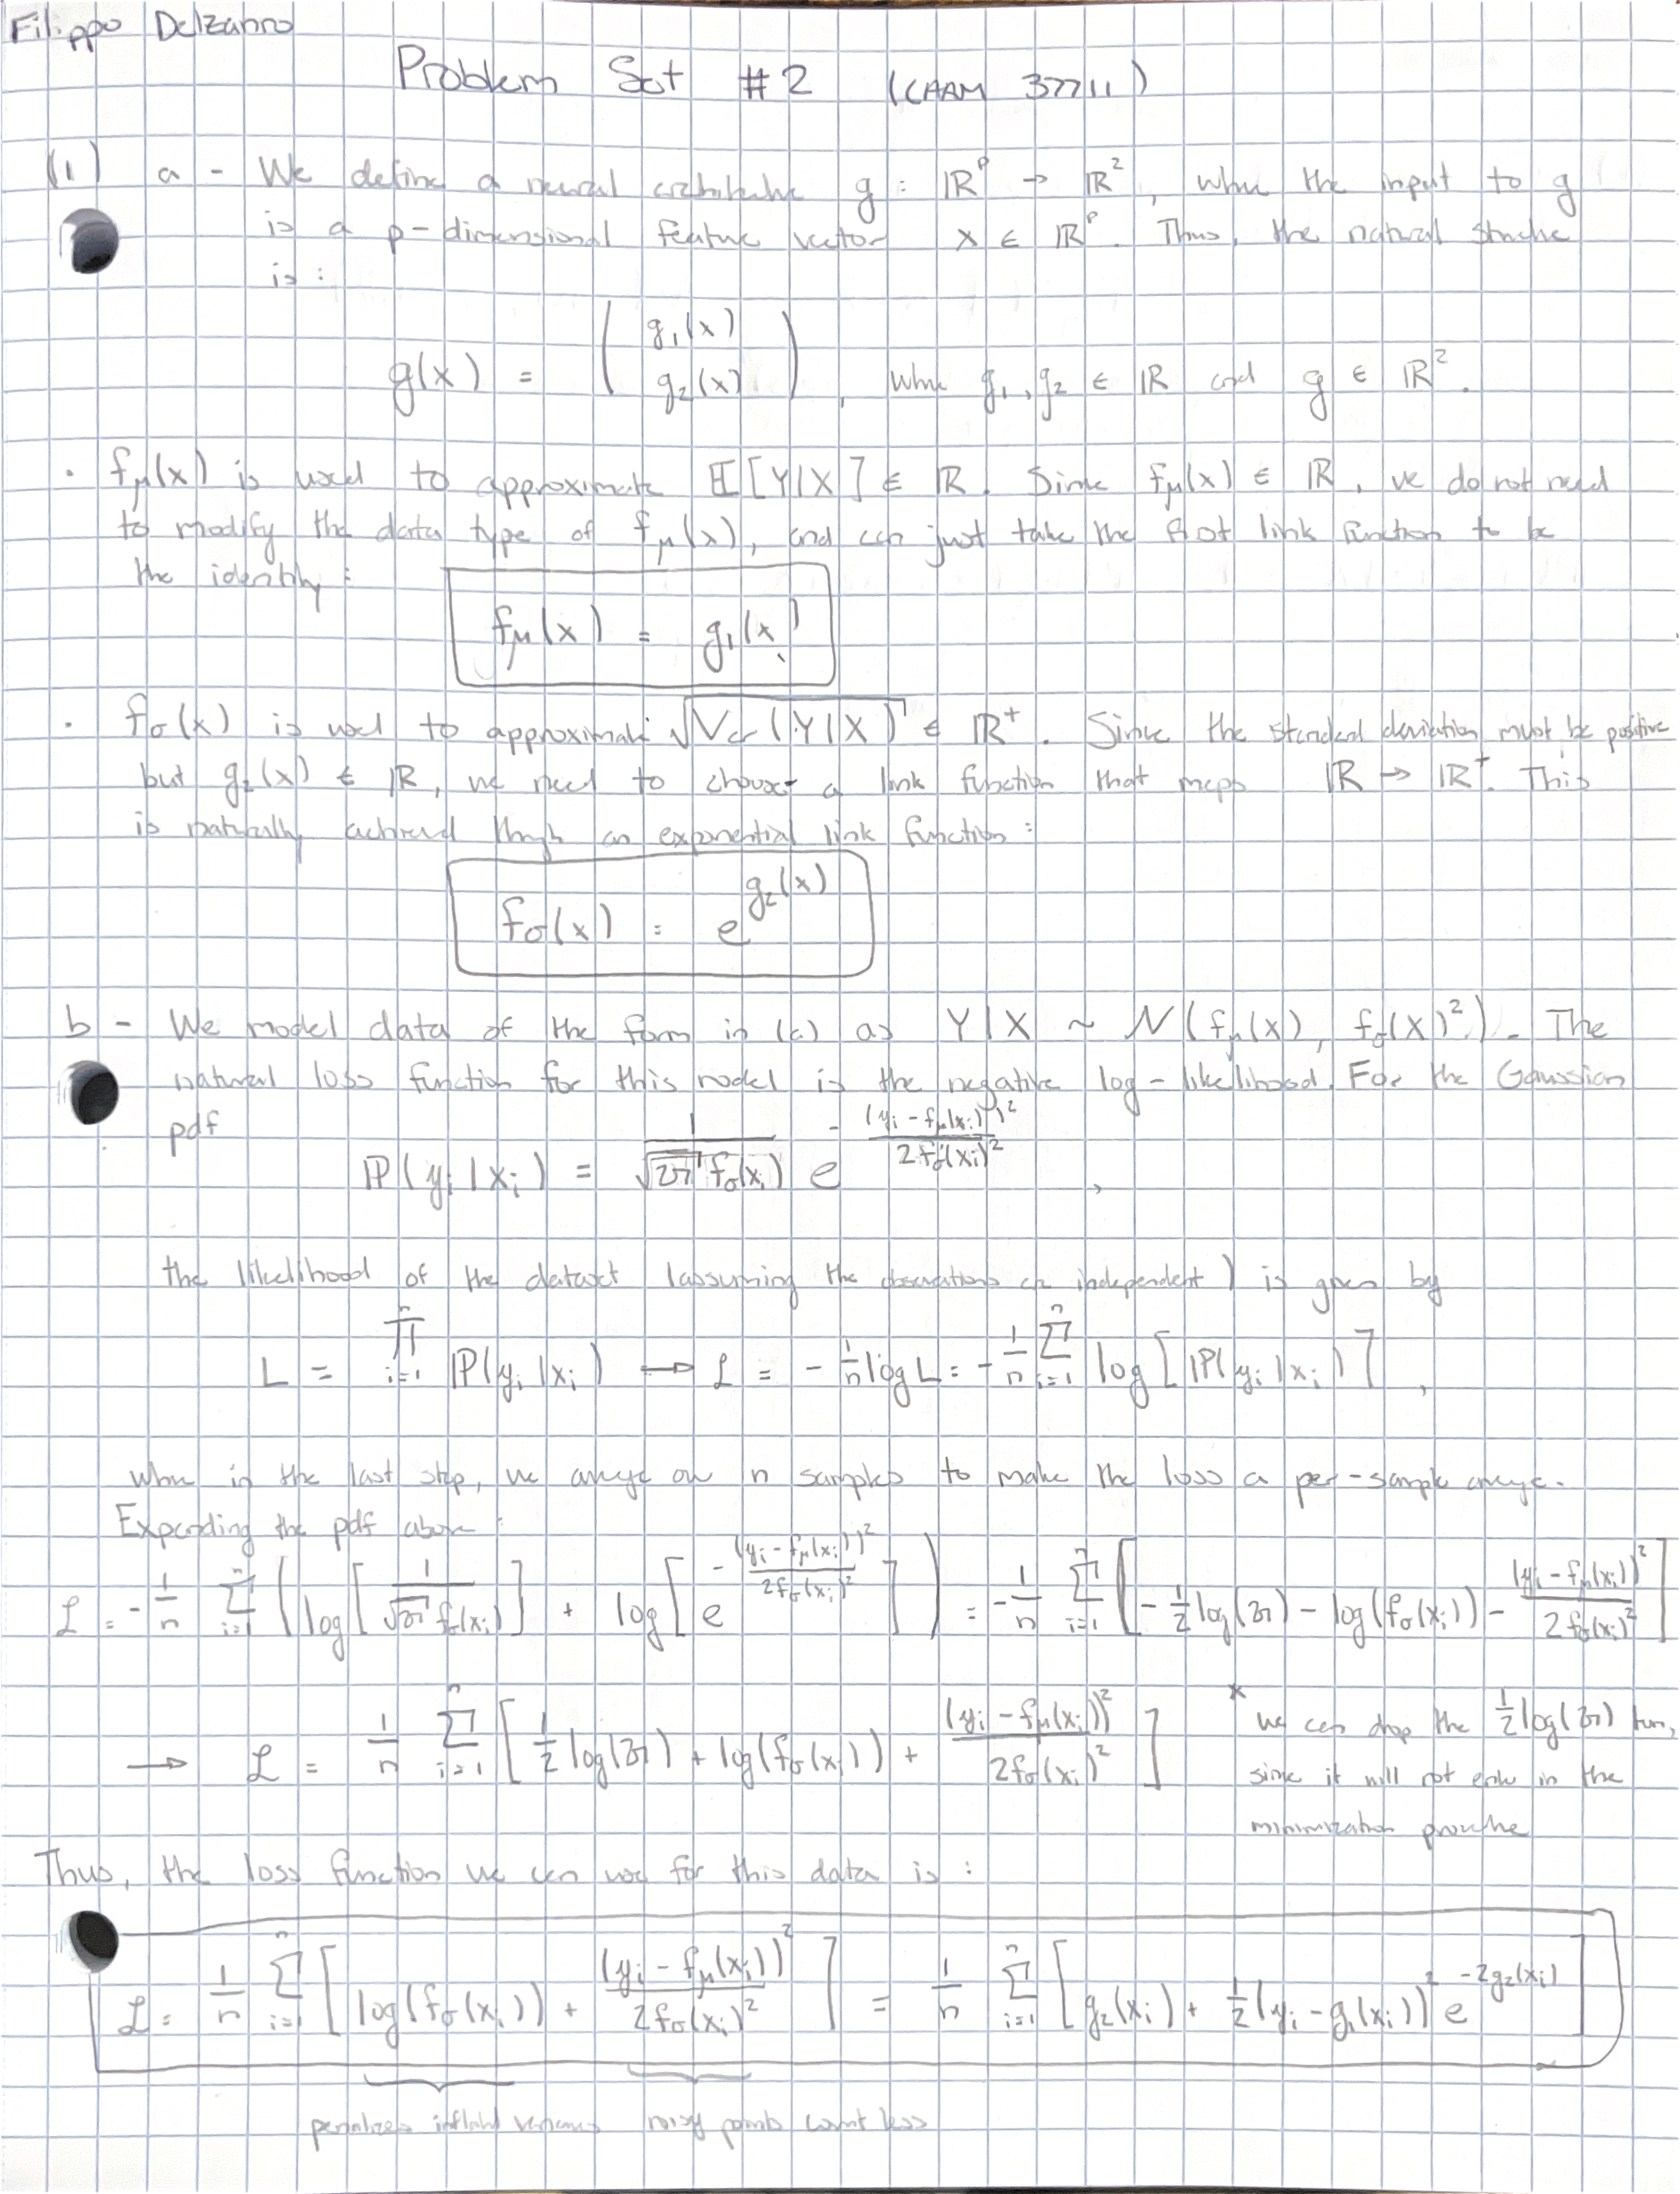
\includepdf[pages=-,pagecommand={\thispagestyle{empty}}]{theory/P1_abcd.pdf}%
}{%
  \bigskip\noindent\textbf{[Handwritten solutions not yet added: place the scan at
  \texttt{homework-2/report/theory/P1\_abcd.pdf} and rebuild.]}%
}

All code for this assignment is in the GitHub repository \url{https://github.com/fdelzanno/CAAM-37711}, under the \texttt{homework-2/} directory. See \texttt{README.md} for setup and run instructions.

\section*{Problem 1}

\subsection*{(c) Model, baselines, and results}

We choose to model $\log$(trip duration) to ensure that probability is never assigned to trips with negative durations and split the data 70/15/15 into training, validation, and test sets. We also standardized and clipped the features using training-set statistics. The network is a ReLU MLP with hidden layers (128, 128, 64) where the first output is the mean $\mu(x)$, and the second is passed through $\sigma(x) = e^{g_2(x)}$ (to keep the standard deviation positive). We train by minimizing the Gaussian negative log-likelihood from (b) and use mini-batch SGD with gradient-norm clipping, a learning-rate scheduler that reduces the rate on plateaus, and early stopping on validation loss. The model is compared against four baselines: a constant model, which predicts the training mean and variance, along with linear regression, gradient boosting, and an MLP trained with MSE loss, each predicting a mean (with one constant variance taken from their validation residuals). All models are evaluated on the held-out test set using NLL, RMSE, and MAE, and the (empirical) coverage of the 68\% and 95\% intervals (used to determine whether the model's uncertainty estimates are accurate).

\begin{table}[h]
  \centering
  \input{\results{p1_metrics_table.tex}}
  \caption{Test-set metrics for each model on $\log(\text{trip duration})$. NLL is the mean Gaussian negative log-likelihood, RMSE and MAE are in log-minutes, MAE (min) is in minutes, and Cover $q\%$ is the fraction of test points within the central $q\%$ predictive interval.}
  \label{tab:p1-metrics}
\end{table}

The Gaussian-NLL MLP and gradient boosting are the best predictors, with an MAE of about 2.3 minutes versus 4.6 for linear regression and 5.6 for the constant model. The MSE-trained MLP is slightly worse. The nonlinear models are therefore capturing structure that a linear fit cannot. The Gaussian-NLL MLP’s advantage shows up in the NLL, since its MAE is essentially tied with gradient boosting. This is likely because it learns an input-dependent $\sigma(x)$, which the baselines cannot learn. The coverage results support this: the 68\% intervals of linear regression, gradient
boosting, and the MSE-trained MLP cover 73–79\% of test points — so they are too wide for typical
trips, likely because a few large residuals inflate the constant variance — while the Gaussian-NLL
MLP covers 70.2\%, close to the expected 68\%.

\subsection*{(e) Evaluation of the predicted probabilities}

For each model, we computed the predicted probability that a test trip takes under 45 minutes (from the formula in part (d)) and compared it to the observed 0/1 label. As a proper scoring rule, we report both the Brier score --- the mean squared difference between the predicted probability and the outcome --- and the log-loss --- the mean negative log-likelihood of the observed labels. Accuracy is obtained by predicting \enquote{under 45 minutes} whenever the probability is at least 0.5 and comparing it to the true label. Since almost every trip is short (99.55\% take under 45 minutes), always predicting \enquote{under 45 minutes} already achieves 99.55\% accuracy. This serves as the reference point.

\begin{table}[h]
  \centering
  \input{\results{p1_prob_table.tex}}
  \caption{Test-set Brier score, log-loss, and accuracy for $P(\text{trip} < 45\text{ min})$.}
  \label{tab:p1-prob}
\end{table}

We see that accuracy is nearly saturated and cannot effectively distinguish the models. The constant model only ties the trivial predictor, and linear regression does worse. The nonlinear models, however, gain only about a tenth of a percentage point. The Brier score and log-loss are more useful: both rank linear regression worst, with gradient boosting, the MLP with MSE loss, and the Gaussian-NLL MLP far ahead of the constant and linear baselines. The Gaussian-NLL MLP has the lowest Brier score, although gradient boosting has the lowest log-loss and the highest accuracy. Since the differences among these three are very small, it is difficult to say with any certainty which model performs best.

\section*{Problem 2}

\subsection*{(a) Cardinality of the features and data splits}

\begin{table}[h]
  \centering
  \input{\results{p2_cardinality_table.tex}}
  \caption{Cardinality of the categorical features and the number of rows in which each unique value appears.}
  \label{tab:p2-card}
\end{table}

From the table above, we can comment on the cardinality of the features. StockCode has 3,665 unique values and CustomerID has 4,339, across 397,924 rows. Both features are high-cardinality and demonstrate uneven category sizes: the median category appears in only 49 rows for StockCode and 41 for CustomerID, while the largest appears in 2,035 and 7,847 rows, respectively. 548 stock codes (about 15\%) and 300 customers (about 7\%) appear in five or fewer rows. We could perform a one-hot encoding, but the large number of categories makes it impractical. It would create 8,004 columns (3,665 + 4,339) and require a dense float64 matrix of about 25.5 GB, almost entirely comprised of zeros. Even with a sparse representation, a model would have to learn a separate weight for each category, which becomes an issue for rare categories where there is almost no data to learn from. This suggests encodings that compress each category into a few representative numbers.

\begin{table}[h]
  \centering
  \input{\results{p2_unseen_table.tex}}
  \caption{Number of validation and test rows whose category never appears in the training set.}
  \label{tab:p2-unseen}
\end{table}

We randomly split the data into training, validation, and test sets (70/15/15\%). Note that this inevitably leads to some rare categories appearing only in validation or test. We quantify this in Table~\ref{tab:p2-unseen}: 30/48 StockCode rows and 19/23 CustomerID rows in the validation/test sets (respectively) have a category not seen in training. Our model will still need to produce a prediction for these rows. The validation set is used for early stopping when training the neural network models in parts (c) and (d), and the test set is held out for final evaluation.

\subsection*{(b)--(d) Target encoding, embeddings, and the combined model}

\begin{table}[h]
  \centering
  \input{\results{p2_metrics_table.tex}}
  \caption{Poisson deviance (train, validation, test), and test MAE and RMSE for the mean baseline, the target-encoding model, the embedding network, and the combined network.}
  \label{tab:p2-metrics}
\end{table}

\textbf{(b)} To implement target encoding, we replace each category with its (smoothed) mean \texttt{Quantity} from the training set. Since \texttt{Quantity} is a positive integer (count) that is heavy-tailed, we fit a gradient-boosting model with a Poisson loss. We also cap the training target at the 99.9th percentile to stop a few huge counts from destabilizing the fit. This result is much better than the baseline that predicts the training mean: test deviance (the Poisson-loss counterpart of mean squared error) falls from 25.86 to 8.38, MAE from 12.63 to 7.14, and RMSE from 37.06 to 28.11.

\textbf{(c)} To develop an embedding neural network, we first need to assign every stock code and every customer a list of 16 numbers. These numbers are adjusted by the network during training. Then, the two learned embeddings are fed into a one-hidden-layer network (64 units) whose output is the log of the predicted \texttt{Quantity}. We train this network with Poisson loss, and find that it beats target encoding on every metric: test deviance is 6.81 vs. 8.38, MAE is 6.22 vs. 7.14, and RMSE is 27.63 vs. 28.11. This difference likely stems from the flexibility of the embedding. By tuning directly on the training data, it is likely to improve the final prediction compared to target encoding, which must summarize each category by one fixed number.

\begin{table}[h]
  \centering
  \input{\results{p2_seeds_table.tex}}
  \caption{Embedding and combined networks refit under five random seeds (the seed used above plus four more with the same data split). Entries are mean $\pm$ standard deviation across seeds. The last row is the paired per-seed difference (Combined $-$ Embeddings).}
  \label{tab:p2-seeds}
\end{table}

\textbf{(d)} To develop the combined model, we feed the embeddings and the two target-encoded features into the same neural network. We find that it beats target encoding (test deviance 6.98 vs. 8.38) but not the embeddings alone. It is also slightly worse on deviance (6.98 vs. 6.81) and MAE (6.41 vs. 6.22), but slightly better on RMSE (27.00 vs. 27.63). To identify whether this was a true shortcoming of the combined model, we trained the same network across five seeds (i.e., across 5 random initializations with the data split held fixed), with those results in Table~\ref{tab:p2-seeds}. We found that the paired difference (Combined $-$ Embeddings) is $0.05 \pm 0.11$ in test deviance and $0.10 \pm 0.11$ in test MAE. Since both are within noise, we see that adding target encoding to the embedding has no clear advantage. This seems plausible, given that the embeddings can already learn (from the training data) information that the target-encoded means contain.

\subsection*{(e) Intuition for the results}

\begin{table}[h]
  \centering
  \input{\results{p2_mae_stockcode_table.tex}}
  \caption{Test MAE by number of training rows for the test row's \texttt{StockCode}.}
  \label{tab:p2-mae-stock}
\end{table}

\begin{table}[h]
  \centering
  \input{\results{p2_mae_customerid_table.tex}}
  \caption{Test MAE by number of training rows for the test row's \texttt{CustomerID}.}
  \label{tab:p2-mae-cust}
\end{table}

Intuitively, this type of problem is well-suited for an embedding layer. Consider that an embedding layer associates each category with a short list of learned numbers that serves as its \enquote{profile}. The network then tunes these profiles to improve its predictions. Since retail data can contain features with thousands of categories, embedding gives a useful strategy for associating categories that behave alike --- such as products bought in similar amounts or customers who order in similar ways --- with similar profiles. The profile can hold more information than a single representative number (such as the average) for a category, and the network is also able to combine the stock-code and customer profiles. We see this complementarity paying off on the test set, where the embeddings reached much better accuracy than the target encoding.

To figure out where the gains in using embeddings come from, we can construct the MAE-by-frequency tables above. For categories seen more than five times in training, embeddings beat target encoding for both features. Rare categories, however, behave differently. For StockCode seen five or fewer times, embeddings are worse than target encoding. We can understand this in the framework we described above: profiles learned from few rows of data are unreliable, while target encoding's smoothing pulls these categories toward the overall mean. In these cases, we can expect the accuracy of an embedding model to worsen. For rare CustomerID, embeddings still perform better, but we should note that all models, including the baseline, do poorly in this category. The combined model has no clear advantage on rare categories, but seems to perform slightly worse than embeddings alone on medium and common categories. We can justify this by recalling the seed results from part (d), which showed no clear gain from adding target encoding. Again, this is likely because an embedding network learns the information captured by target encoding along the way. Overall, rare categories comprise less than 1\% of the test rows, so they barely affect the overall numbers.

\section*{Problem 3}

\subsection*{(a) Data visualization}

\begin{figure}[h]
  \centering
  \includegraphics[width=\textwidth]{\results{figures/p3_training_data.png}}
  \caption{Training data: $(x_1,x_2)$ colored by $y$ (left) and $y$ on the vertical axis (right).}
  \label{fig:p3-data}
\end{figure}

\subsection*{(b) Random Kitchen Sinks with ridge regression}

We implemented a Random Kitchen Sink model by drawing $h = D/2$ random projections with weights $W$ drawn i.i.d. from $\mathcal{N}(0, \sigma^{-2})$ and phases $b \sim U[0, 2\pi]$. Each input is mapped to the $D + 1$ features $[\sin(W^{T}x + b), \cos(W^{T}x + b), 1]$, and the linear weights are fit by ridge regression. We chose to vary the number of random features $D \in \{10, 20, 50, 100, 200, 500, 1000, 2000\}$ as our hyperparameter, keeping the kernel scale ($\sigma = 1$) and the ridge strength ($\lambda = 10^{-3}$) fixed. For each $D$, we fit on the training set and record the training and validation MSE.

\begin{figure}[h]
  \centering
  \includegraphics[width=\textwidth]{\results{figures/p3_rks_sweep.png}}
  \caption{RKS training MSE (left) and validation MSE (right) as a function of the number of random features $D$. The dashed line marks the best $D$ on validation.}
  \label{fig:p3-rks}
\end{figure}

\begin{table}[h]
  \centering
  \input{\results{p3_rks_sweep_table.tex}}
  \caption{RKS sweep over the number of random features $D$.}
  \label{tab:p3-rks}
\end{table}

We find that small $D$ tends to underfit, but the training and validation MSE both fall sharply by $D = 50$. After that, the training MSE plateaus, decreasing only slightly through $D = 2000$. We see that the validation MSE reaches its minimum at $D = 50$ and then rises slowly for larger $D$. This increasing train--validation gap is likely an indicator of mild overfitting. By selecting on validation loss, we take $D = 50$ as our optimal hyperparameter, but note that the differences between $D = 50$--$200$ are small --- indicating that the model is not very sensitive to $D$ past an initial underfitting regime.

\subsection*{(c) One-hidden-layer MLP}

We fit a one-hidden-layer MLP in PyTorch with a ReLU activation, so the network maps $x$ through a linear layer of width \texttt{d\_hidden}, then a ReLU, then a linear output layer. It is trained by minimizing the MSE loss with mini-batch SGD (using a learning rate of $10^{-2}$, batch size 128, 2000 epochs). We chose to vary the hidden layer dimension $\texttt{d\_hidden} \in \{2, 4, 8, 16, 32, 64, 128, 256, 512\}$ as our hyperparameter, keeping the learning rate, batch size, number of epochs, and activation fixed. For each \texttt{d\_hidden}, we fit on the training set and record the training and validation MSE.

\begin{figure}[h]
  \centering
  \includegraphics[width=\textwidth]{\results{figures/p3_mlp_sweep.png}}
  \caption{MLP training MSE (left) and validation MSE (right) as a function of the hidden layer dimension. The dashed line marks the best dimension on validation.}
  \label{fig:p3-mlp}
\end{figure}

\begin{table}[h]
  \centering
  \input{\results{p3_mlp_sweep_table.tex}}
  \caption{MLP sweep over the hidden layer dimension.}
  \label{tab:p3-mlp}
\end{table}

We find that very small networks tend to underfit, but the training and validation MSE both fall sharply by $\texttt{d\_hidden} = 8$. Beyond that, the training MSE keeps decreasing slowly while the validation MSE plateaus. The validation MSE reaches its minimum at $\texttt{d\_hidden} = 256$ and is essentially unchanged for higher \texttt{d\_hidden}. By selecting on validation loss, we take $\texttt{d\_hidden} = 256$ as the optimal hyperparameter, but note that the differences in validation MSE for $\texttt{d\_hidden} \geq 16$ are small --- indicating that the model is not very sensitive to \texttt{d\_hidden} once it has enough capacity. Unlike RKS, the validation curve does not rise noticeably for larger \texttt{d\_hidden}, so there is no evidence of overfitting.

\subsection*{(d) Comparison and visualization}

\begin{table}[h]
  \centering
  \input{\results{p3_comparison_table.tex}}
  \caption{Validation MSE of the two models refit with their best hyperparameters.}
  \label{tab:p3-compare}
\end{table}

After refitting both models with the selected hyperparameters, RKS ($D = 50$) reaches a validation MSE of 0.0381, and the MLP ($\texttt{d\_hidden} = 256$) reaches 0.0396. Although RKS performs slightly better, the difference is small and each number comes from a single random initialization, so it is reasonable to conclude that the two models are essentially comparable on this data set. However, RKS needed only 50 random sinusoidal features and a closed-form ridge solve, while the MLP needed a hidden layer five times wider and 2000 epochs of SGD just to reach a similar error. This difference in complexity is consistent with the data: the underlying function looks smooth, low-frequency, and has just two inputs, suggesting that sinusoidal features are a good match. The MLP, on the other hand, has to learn its features by stochastic gradient descent, a less direct method that also depends on optimization settings. We would expect an MLP to have the advantage on less smooth or higher-dimensional problems, but that does not apply to this data set. We save the predictions for the unlabeled \texttt{test.csv} in \texttt{rks\_test\_predictions.csv} and \texttt{mlp\_test\_predictions.csv}, one row per test point in the original order.

\begin{figure}[h]
  \centering
  \includegraphics[width=0.48\textwidth]{\results{figures/p3_rks_surface.png}}\hfill
  \includegraphics[width=0.48\textwidth]{\results{figures/p3_mlp_surface.png}}
  \caption{Fitted surfaces over $[-3,3] \times [-3, 3]$ for the RKS model (left) and the MLP (right), each with its best hyperparameter.}
  \label{fig:p3-surfaces}
\end{figure}

The training data in part (a) (Figure~\ref{fig:p3-data}) shows a valley near $(x_1, x_2) \approx (-1.5, 0)$, where $y$ is about $-1$. Away from it, $y$ rises, with the highest values (about 5) near $(x_1, x_2) \approx (1.5, \pm 3)$ at the top and bottom edges. Both fitted surfaces (Figure~\ref{fig:p3-surfaces}) reproduce this structure: a smooth basin centered near the same location, values increasing toward the top and bottom edges, and a saddle near $(x_1, x_2) \approx (1.5, 0)$ separating the valley from a second shallow dip along the right edge. The two surfaces are very similar in range and shape, which is consistent with their near-identical validation MSE. They differ mainly in smoothness. The RKS surface is smoother because it is built from a sum of sinusoids, while the MLP contours are slightly rougher. That jaggedness is the piecewise-linear signature of a ReLU network, which builds the surface from many linear pieces.

\clearpage

\end{document}
